\chapter{Inleiding}
Dit is het Onderzoeksverslag voor het \qw{Het CMS voor iedereen} project.
Het onderzoeksverslag is een onderdeel van de afstudeerperiode binnen NHL Stenden Hogeschool.
Het Onderzoek wordt uitgevoerd bij Snakeware New Media B.V. en is de \textit{requirement analyse} van de \gls{SDLC} (zie figuur \ref{fig:SDLC}).
Dit onderzoek zal gebruik maken van de methodiek uit het boek \textit{Wat is onderzoek} \Parencite{Verhoeven}.

\whitespace
\begin{graphic}
    \vspace{0.2cm}
    \captionsetup{type=figure}
    \caption{De Software development lifecyle afkomstig uit de afstudeer handleiding \Parencite{Afstudeerhandleiding}}
    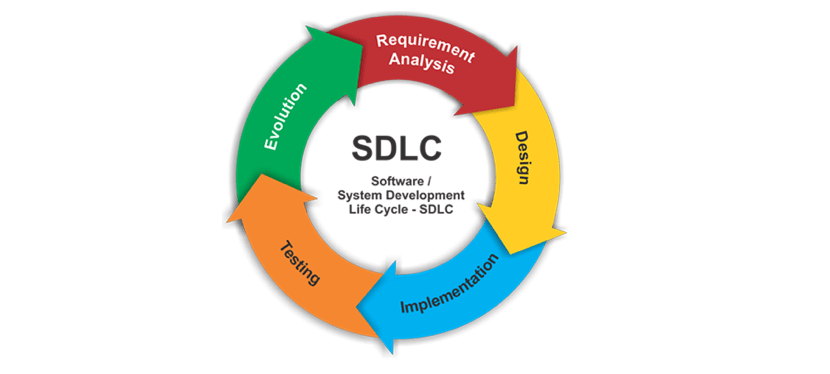
\includegraphics[scale=0.5]{img/SDLC.png}
    \label{fig:SDLC}
    \vspace{0.2cm}
\end{graphic}

\whitespace
In het volgende hoofdstuk wordt de organisatie beschreven verder wordt de aanleiding en de context van de afstudeeropdracht beschreven.

\section{Organisatieomschrijving}
Snakeware New Media B.V. (Snakeware) is een E-business bureau gevestigd in Nederland.
Haar aangeboden diensten omvatten het adviseren, bouwen en onderhouden van digitale
producties, met een focus op websites, webshops en mobiele apps \Parencite{SnakewareWhatWeDo}. Op
het moment van schrijven telt Snakeware meer dan 60 werknemers, elk met verschillende
specialiteiten. Ze leveren services aan welbekende organisaties zoals DPG Media, DekaMarkt
en Poiesz supermarkten \Parencite{SnakewareCases}.
% Snakeware heeft een platform genaamd \qw{Snakeware Cloud} dit platform is een contentmanagementsysteem
% (CMS) Waarmee ze digitale content kunnen leveren voor haar klanten.
% Alle klanten die via Snakeware hun webapplicatie hebben maken gebruik van het Snakeware Cloud platform.
% \whitespace
% \todo[inline]{pictogram referentie maken van de bedrijfs structuur van Snakeware}


\section{Context}
Snakeware heeft een platform genaamd “Snakeware Cloud” dit platform is een \gls{CMS} waarmee ze digitale content kunnen leveren voor haar (grotere) klanten.
Snakeware cloud is een applicatie waarmee Snakeware en haar klanten webapplicaties kan inrichten en voorzien van content.% \todo[inline]{Het is nog niet duidelijk wat het CMS exact doet.
% 	Hoe het nu staat geschreven wordt ook niet duidelijk dat klanten zelf kunnen interacteren met het CMS.
% 	Dit is belangrijke context en moet nog opgeschreven worden (kan ook doormiddel van afbeeldingen).}
\whitespace
De klant van Snakeware kan zijn of haar website zelf inrichten door middel van het specificeren van de content op de verschillende pagina's.
Dit wordt gedaan door middel van artikelen die door het \gls{CMS} gebruikt kunnen worden.
De content van het artikel kan verschillen tussen simpele text, vragenlijst, webshop items, etc.
Hiernaast zijn er ook \gls{SEO} opties binnen Snakeware cloud om de site goed te kunnen vinden op het internet.
Hierbij kun je denken aan URL-optimalisatie binnen het gebruik van de websites.
Hierom heeft Snakeware cloud veel features en configuratie stappen wat het complex en duur maakt om een relatief kleine webapplicatie te maken voor kleinere klanten.
\whitespace
Dit zorgt ervoor dat Snakeware zich niet kan vestigen in een markt met veel kleinere klanten,
en hierdoor omzet mis loopt.
% Het huidige platform is ontworpen om webapplicaties voor grote klanten te ontwik-
% kelen.\todo[inline]{het klinkt nu als of het een tool is (net zo als vs studio) misschien iet neerzetten voor content en dat soort dingen}
% Hierom zijn er veel features en configuratie stappen wat het complex en duur maakt
% om een relatief kleine webapplicatie te maken voor kleinere klanten.
% De klant (of Snakeware) kan de website inrichten doormiddel van het specificieeren van de content op de verschillende paginas.
% Dit wordt gedaan doormiddel van artikelen hierdoor kan een klant zijn eignen content specificieeren en op hun eigen site neer zetten.
% De content kan verschillen tussen simpele text, vragenlijsten, webshops, ect.
% Hiernaast zijn er ook veel SEO opties binnen Snakeware cloud om de site goed te vinden op het internet.
Dit zorgt ervoor dat Snakeware zich niet kan vestigen in een markt met veel kleinere klanten, en hierdoor omzet mis loopt.
 % huidige en gewenste situatie
\section{Aanleiding}
Het huidige platform is 21 jaar oud en er is veel functionaliteit in de loop der jaren aan toegevoegd.
Omdat Snakeware Cloud een oud platform is zijn er veel technieken en best practices gebruikt die nu niet meer als optimaal worden beschouwd.
Deze technieken waren erg geïntegreerd in Snakeware cloud en er is het verleden gekozen om niet de code herschrijven om het aan de huidige standaarden te voldoen van andere projecten.
Een voorbeeld hiervan is tabel naam afkortingen achter elke kolom zetten, of gigantische C\# \Parencite{CSharp} files van 10 000 regels met verschillende functies.
Deze functies houden zich niet aan de \textit{Single Responsibility Principle} van de SOLID ontwerpmethode \Parencite{SOLID} wat het moeilijk maakt om het huidige \gls{CMS} te onderhouden.

\whitespace
Ook zijn er technieken toegepast die nu niet meer relevant zijn.
Een voorbeeld hiervan is dat het \gls{CMS} gebruikmaakt van JavaScript \Parencite{JavaScript} en toen ze er mee begonnen bestonden JavaScript classes \Parencite{JavascriptClasses} nog niet, dus hebben ze die zelf geïmplementeerd.
Deze oudere technieken en standaarden zorgen ervoor dat het meer tijd kost om het CMS te onderhouden vanwege de extra code.
Dit zorgt ervoor dat het meer tijd en geld kost om het Snakeware cloud uit te breiden.
\todo[inline]{ik wou graag bloat gebruiken inplaats van extra code maar volgens kan dat niet suggesities}
% Deze oudere technieken zorgen voor veel overhead en zorgt ervoor dat het veel tijd en geld kost om het \gls{CMS} uit te breiden.

\whitespace[2]
Een van de voornaamste kwesties met Snakeware Cloud betreft de verouderde datastructuur van de applicatie.
Deze veroudering is het gevolg van een initïele ontwikkeling waarbij onvoldoende rekening werd gehouden met toekomstige functionaliteitsuitbreidingen in het systeem.
Als gevolg daarvan is de onderliggende datastructuur niet aangepast, maar zijn er elementen aan toegevoegd.
Dit heeft geresulteerd in database queries van duizenden regels en complexe relaties tussen tabellen in de database.
Dit huidige scenario bemoeilijkt aanzienlijk het toevoegen van nieuwe functionaliteiten, wat resulteert in aanzienlijke tijds- en kosteninvesteringen.

\whitespace[2]
Hierom wildt Snakeware dat er een nieuwe datastructuur komt met daar bij een \gls{CMS}-API.
Omdat er een nieuwe datastructuur moet komen en de logica van het oude systeem nauw verbonden is met de datastructuur is het niet mogelijk om de oude code opnieuw te kunnen
gebruiken.

\section{Opdrachtomschrijving}
\label{sec:Opdrachtomschrijving}
De opdracht is om een proof of concept CMS-API te ontwikkelen die gebruikt maakt van een datamodel en systeemarchitectuur dat flexibeler, onderhoudbaarder is en gebruik maakt van moderne best practices.
Tijdens de afstudeeropdracht wordt er primair op het datamodel en de systeemarchitectuur gefocust.
Omdat er nog geen concreet datamodel en systeemarchitectuur is zal dit onderzocht/ontworpen moeten worden.

\whitespace[2]
De opdracht omvat het achterhalen van de requirements, ontwerpen en ontwikkelen van het proof of concept met als focus een nieuw datamodel, met de essentiële functionaliteiten.

\whitespace[2]
Het huidige Snakeware cloud platform bestaat uit 2 verschillende \gls{GUI}:
\begin{itemize}
	\item[-] Snakeware cloud \gls{GUI}
	\item[-] Klant webapplicatie
\end{itemize}

\whitespace
Met de Snakeware cloud \gls{GUI} kan de klant de content van de website aanpassen.
Door middel van de webapplicatie kan de eindgebruiker de content bekijken en er mee interacteren.
Er is voor gekozen om niet de Snakeware cloud \gls{GUI} te realiseren om de afstudeeropdracht in scope te houden.
Er is wel voor gekozen om de klant webapplicatie in zijn minimale vorm uit te werken.

\whitespace[2]
% Om de \gls{UserJourneys} te testen wordt er gebruikgemaakt van postman workflows \Parencite{PostmanWorkflows}.
Het doel van het proof of concept is dat er aangetoond kan worden dat door het gebruiken van een nieuw datamodel en systeemarchitectuur ook services verleend kunnen worden aan kleinere klanten.
Dit zou eventueel ook een startpunt zijn om op verder te bouwen.

\todo[inline]{Laat zien hoe de userflowes wel getest worden anders ziet er net uit of je niks doet.}
% \todo[inline]{Feedback van justin: \textit{Deze paragraaf is nu niet gepast voor een onderzoeksverslag}}
% \todo[inline]{Misschien een stukje theoretisch kader/ voor onderzoek te hebben waarin je het CMS ietwat toelicht (misscien met plaatje wow) (De pre, zonder je deelvragen te beantwoorden). Ik weet alleen niet of ik hier genoeg tijd voor heb}
%

% \section{Stakeholders}
In het vooronderzoek wordt er een stakeholdersanalyse gemaakt om de stakeholders in beeld te krijgen.
De stakeholders zijn inviduen of organisaties die invloed of belang hebben bij het project, 
omdat het project een proof of concept is zullen er voor de exterene stakeholders gekwalificeerde medewerkers gebruikt worden om de wensen van de klant te kunnen vertegenwordigen

% \todo[inline]{examen comissie:
% \emph{Mits je sirieus onderzoek doet naar de requirements met je "gekwalificeerde interne stakeholders" zou 
% het mogelijk moet zijn je opdracht te kaderen en concreet te maken wat er gemaakt moet gaan worden voor de PoC.
% Toch denken wij dat eht verstandig is om ook een met de eindgebruikers te praten. maak de opdracht niet te groot en niet te klein}}
% \todo[inline]{Wie zijn er betrokken bij dit project? Verwijzen naar bijlage?}
Product owner
Ontwikkelteam
afdeling commercie?
Afdeling R&D
Developers
Ontwikkelteam
Kleine klanten (wordt verantegenwoordigd door ?)
Entreprise klanten (wordt verantegenwoordigd door?)
"normale" klanten (wordt verantegenwoordigd door?)
eindgebruikers (wordt verantegenwoordigd door ?)
\subsection{Interne Stakeholders}
\begin{tabular}{ | p{3cm} | p{9cm} | }
    \hline
    \textbf{Stakeholder} & \textbf{Bescrijving} \\ 
    \hline
    Product owner & De product owner overziet het project en vasiliteerd de communicatie tussen de ontwikkelaars en de klanten \\
    \hline
    Afdeling R\&D  & de afdeling R\&D van Snakeware zijn de ontwikkelaars van het huidige CMS en kunnen veel inzicht bieden in de huidige situatie / problemen.  \\ 
    \hline
    Developers & Aan het einde van de afstudeerperiode moet het project overgedragen worden aan de developers van Snakeware.\\
    \hline
    Ontwikkelteam & Het ontwikkelteam is verantwoordelijk voor het realiseren van het proof of concept\\
    % \hline
    % Afdeling Comercie & hij is heel cool \\
    \hline
\end{tabular}

\subsection{Externe Stakeholders}
\begin{tabular}{ | p{3cm} | p{9cm} | }
    \hline
    \multicolumn{2}{| c |}{Externe Stakeholders} \\
    \hline
    Kleine klanten & goed bescrijving voor kleinere klanten \\
    \hline
    Entreprise klanten & Dit zijn klanten bij Snakeware die een grote hoeveelheid klanten heeft en meestal binnen Snakeware eigen teams heeft, Hierbij kan je denken aan Poieze, DRG en Rederij Doeksen. \\ 
    \hline
    Huidige klanten & De huidige klanten die bij Snakeware een web applicatie hebben.\\
    \hline
    Eindgebruikers & De personen die de content van de verschillende web applicaties gaan inlezen en gebruiken. \\
    \hline
\end{tabular}
\subsection{Invloeds- en belangenmatrix}
plaatje
\subsection{Relatie tussen stakeholders}
plaatje

\section{Leeswijzer}
In hoofdstuk 2 wordt de onderzoeksopzet behandeld hier worden de hoofd- en deelvraag opgesteld.
Daarnaast worden de verschillende onderzoeksmethoden uitgelegd bij elke deelvraag.
In hoofdstuk 3 worden de resultaten van het onderzoek behandeld en geanalyseerd.
In hoofdstuk 4 wordt de conclusie van het onderzoek behandeld en wordt er antwoord gegeven op de hoofdvraag.
In het laatste hoofdstuk wordt de discussie en reflectie behandeld.

